\input texbase

\titulo{Exercício Programa 2}
\materia{MAC300 - Métodos Numéricos da Álgebra Linear}

\aluno{Fernando Omar Aluani}{6797226}

\begin{document}
\cabecalho

\section{Filtros}

%%%%%%%%%%%%%%%%
\subsection{Ajuste do Contraste - Equalização de Histograma}
\subsubsection{Implementação}
O filtro de contraste é implementado equalizando o histograma da imagem. Inicialmente o algoritmo percorre por cada pixel
da imagem para contar o nivel de cinza para construir o histograma. Após isso, a função de distribuição acumulada é 
calculada, armazenando seu resultado para cada nível de cinza em um vetor, e o valor mínimo em uma variável à parte.

Finalmente, a imagem processada é construída, calculando o valor de cada pixel um-a-um, normalizando o histograma.

Caso o programa mostre a comparação das imagens (ver \textit{README}), ele irá mostrar também o histograma da imagem
original e o histograma da imagem processada.

\subsubsection{Vantagens e Desvantagens}
Computacionalmente, dos três filtros apresentados aqui este é o mais eficiente, tendo uma complexidade de somente $O(NM)$
(para uma imagem de tamanho $N\times M$). Em relação à memória, descontando a imagem resultante já que todos filtros 
criam ela, este método não gasta muito, sendo o principal os três vetores com 256 floats que ele guarda internamente.

Quanto ao desempenho como filtro, este é o método no qual a diferença do resultado para a imagem original é mais facilmente
notada. Porém, este filtro pode criar resultados não-realísticos dependendo da imagem original.

\subsubsection{Exemplo}
\begin{figure}[htb]
    \centering
    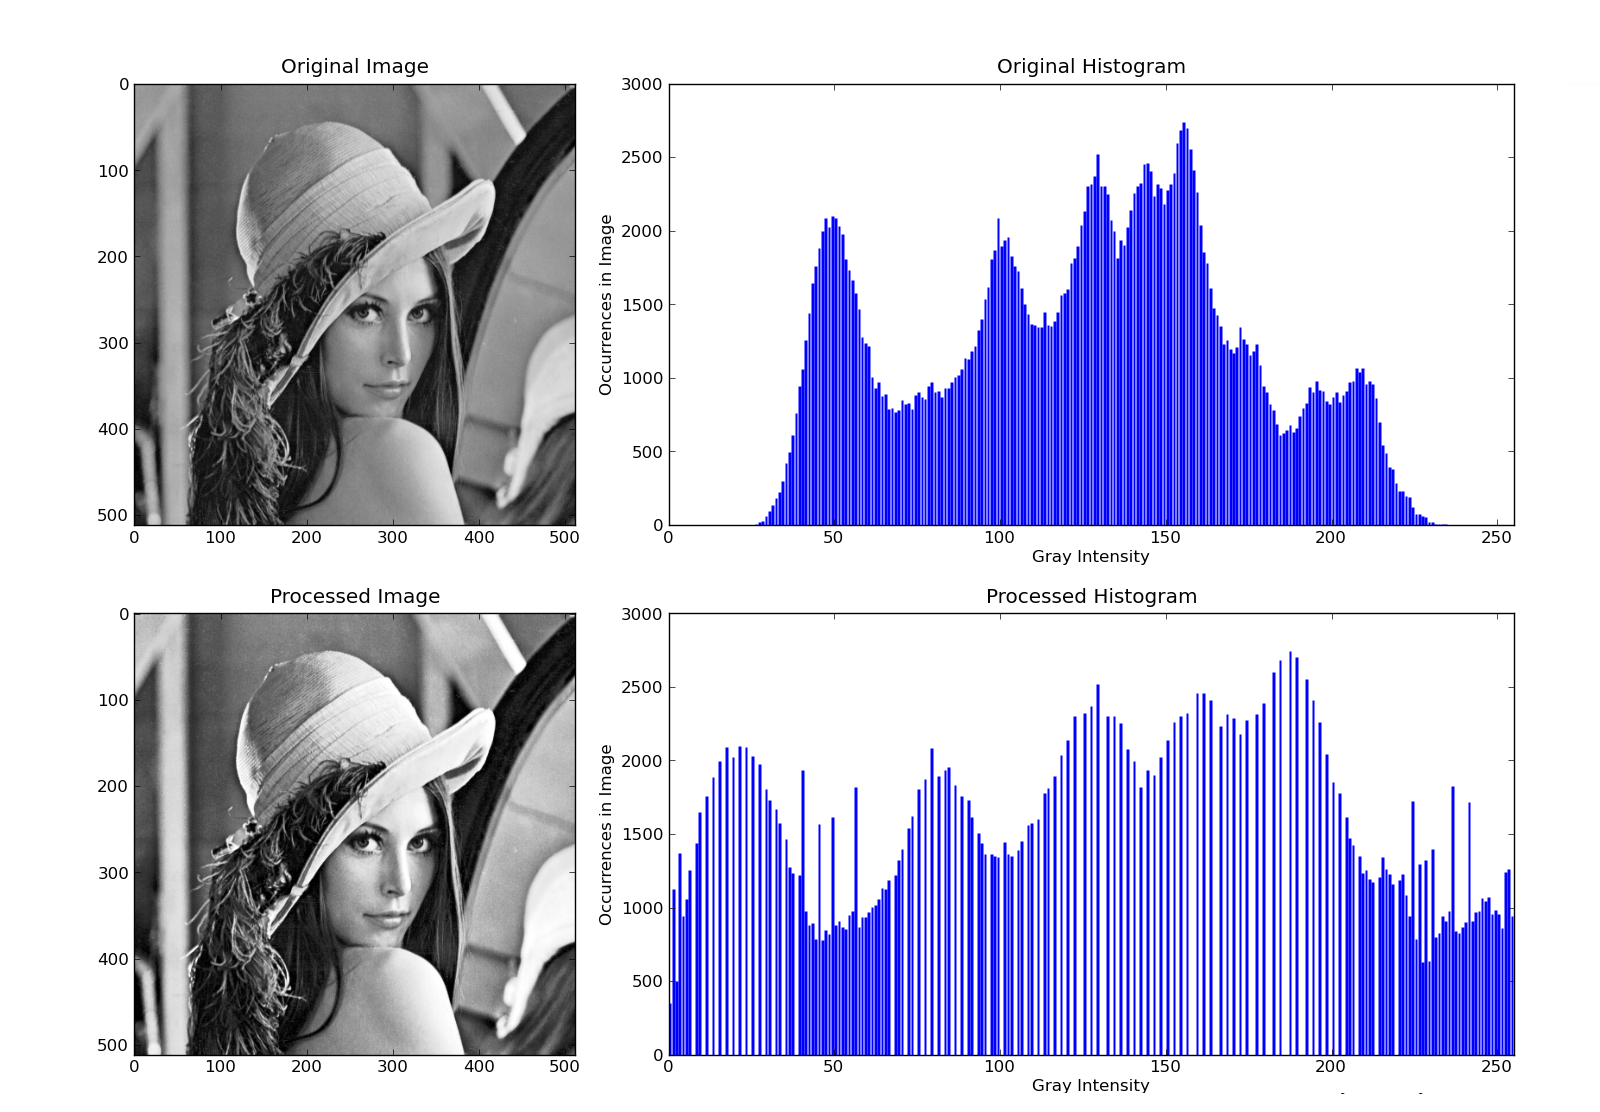
\includegraphics[width=1.0\textwidth]{contrast_example.png}
    \caption{Comparação das imagens (original e após o ajuste de contraste) e seus respectivos histogramas.}
    \label{fig:ex_contraste}
\end{figure}

%%%%%%%%%%%%%%
\subsection{Suavização por Média Ponderada - \textit{Blurring}}
\subsubsection{Implementação}
O filtro de \textit{blur} foi implementado usando a técnica de filtro de convolução, com uma máscara $3\times 3$ para tirar
a média ponderada dos pixeis ao redor do pixel sendo suavizado. O resultado da convolução da imagem já é o resultado
do processamento.

\subsubsection{Vantagens e Desvantagens}
Computacionalmente, este filtro simplesmente aplica a convolução, e ela tem complexidade $O(NMST)$ (Para uma matriz 
$N\times M$, com uma máscara de tamanho $S\times T$). Em relação à memória, ele não tem gasto adicional de memória.

Quanto ao desempenho como filtro, dependendo da imagem original pode ser difícil notar alguma diferença com o 
resultado, e o \textit{blurring} pode ocultar detalhes da imagem.

\subsubsection{Exemplo}
\begin{figure}[htb]
    \centering
    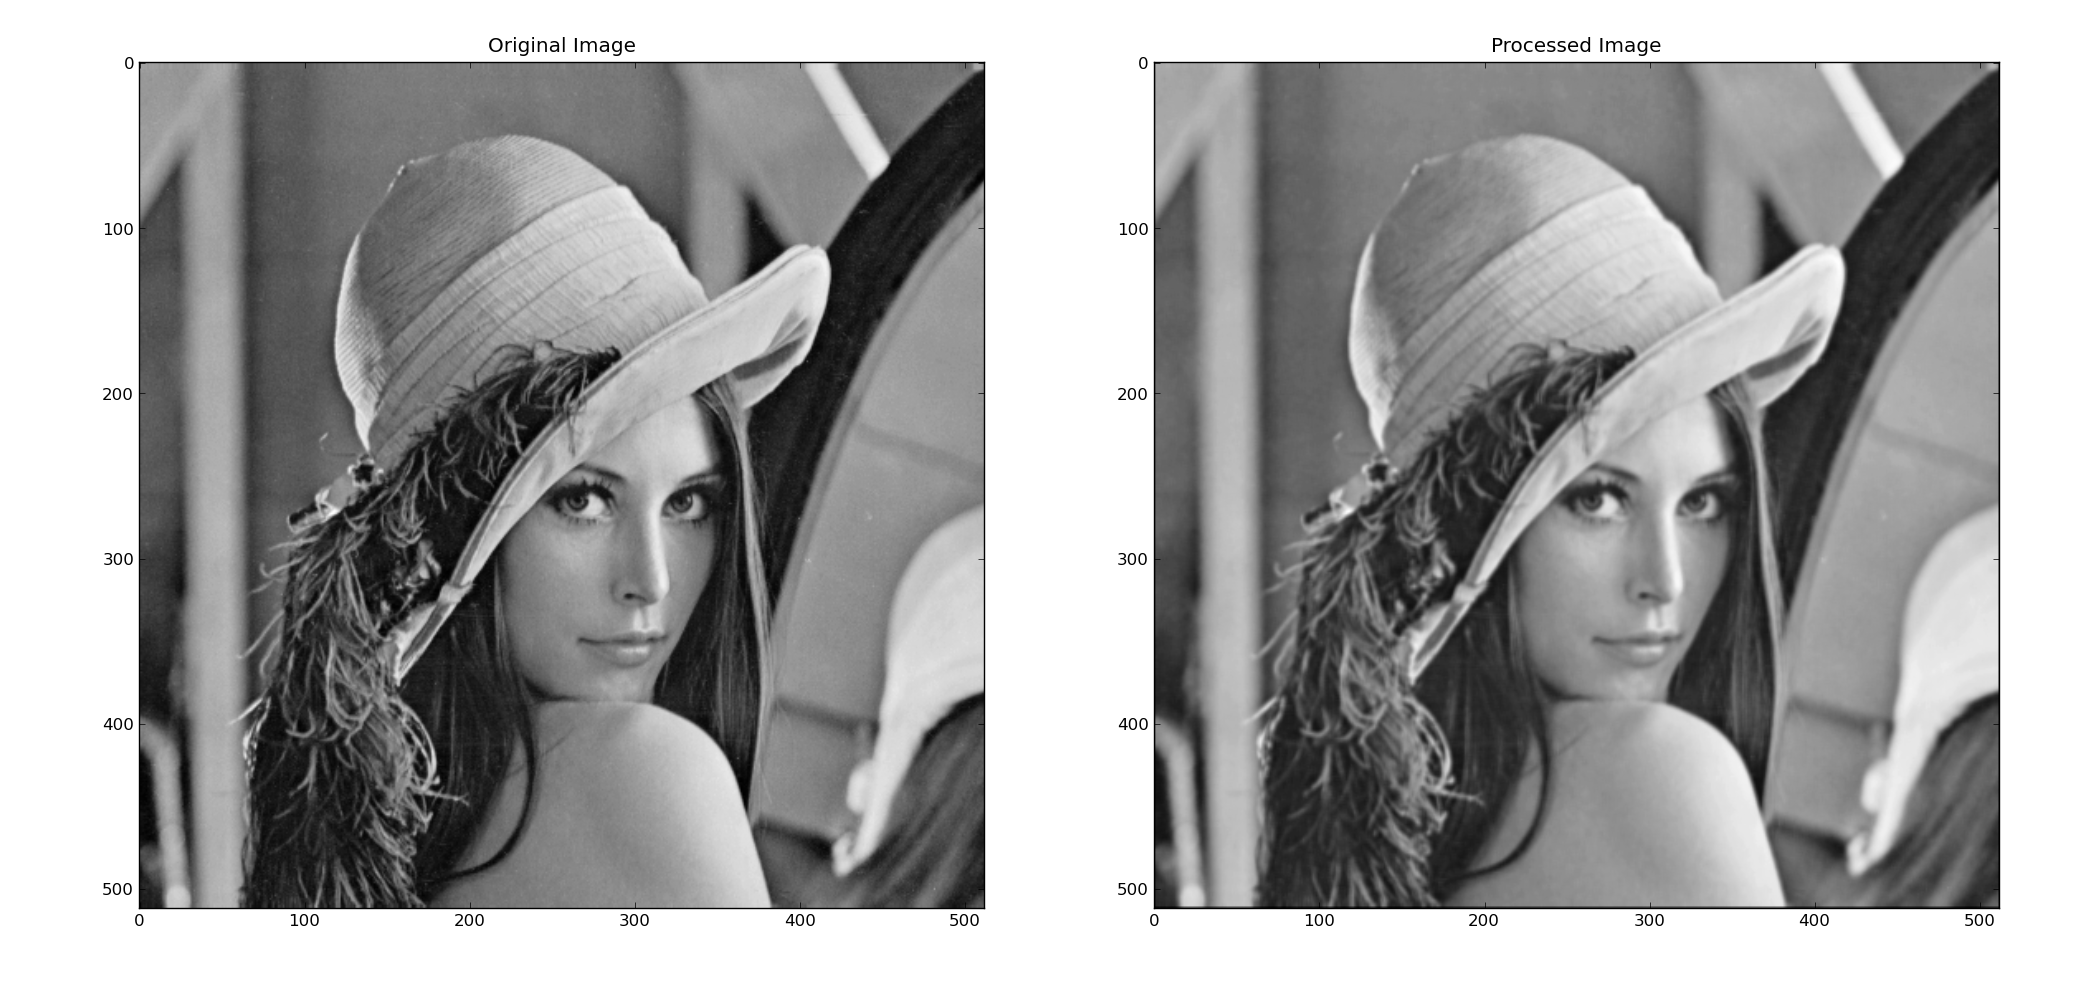
\includegraphics[width=1.0\textwidth]{blur_example.png}
    \caption{Comparação das imagens (original e após o \textit{blurring}).}
    \label{fig:ex_blur}
\end{figure}

%%%%%%%%%%%%%%
\subsection{Aumento de Nitidez - \textit{Sharpening}}
\subsubsection{Implementação}
O filtro de \textit{sharpen} foi implementado usando a técnica de filtro de convolução, com uma máscara $3\times 3$
conhecida como \textit{8 neighbour Laplacian}. Usando a convolução na imagem original adquirimos o resultado do operador
laplaciano na imagem. O resultado final da imagem processada é a soma da imagem original com o laplaciano dela.

Caso o programa mostre a comparação das imagens (ver \textit{README}), ele irá mostrar também a imagem do operador 
laplaciano. 

\subsubsection{Vantagens e Desvantagens}
Computacionalmente, dos metodos apresentados aqui este é o mais pesado. Ele roda uma convolução, que tem complexidade 
$O(NMST)$ (Para uma matriz $N\times M$, com uma máscara de tamanho $S\times T$), e depois ele soma 2 imagens. Em
relação à memória, ele guarda o resultado da convolução - o laplaciano da imagem.

Quanto ao desempenho como filtro, assim como o \textit{blurring}, a diferença no resultado pode ser difícil de notar,
sendo mais fácil ver resultados aplicando o filtro a uma imagem suavizada (pelo \textit{blurring}, por exemplo).

\subsubsection{Exemplo}
\begin{figure}[htb]
    \centering
    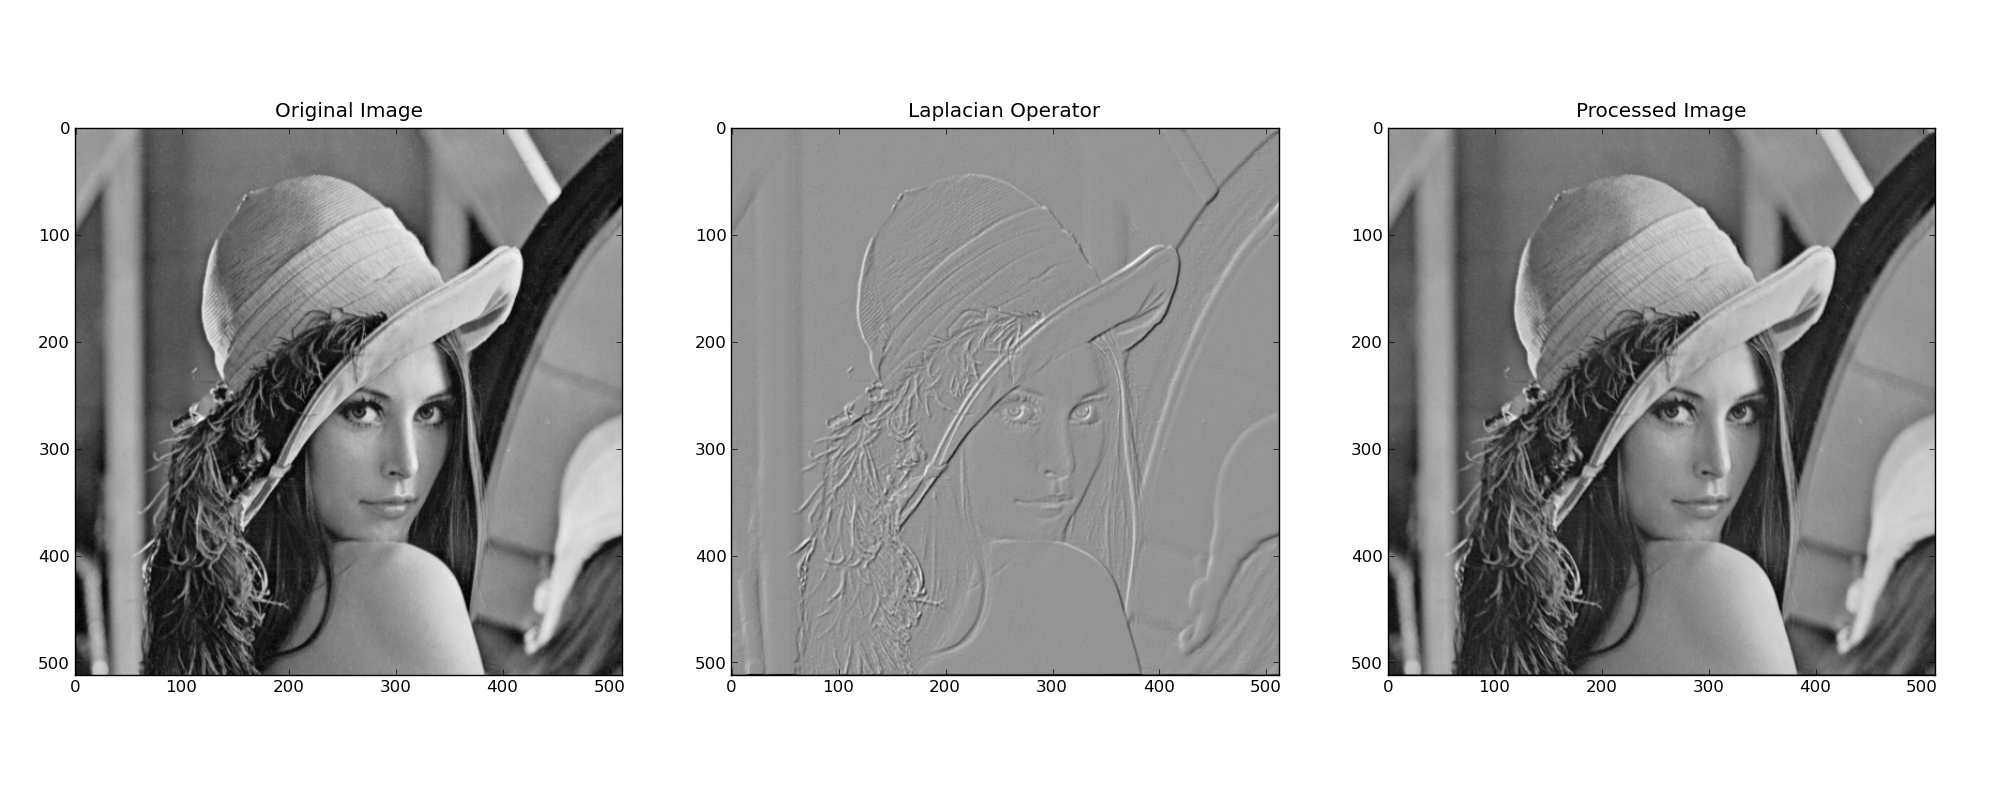
\includegraphics[width=1.0\textwidth]{sharpen_example.png}
    \caption{Comparação das imagens (original e após o \textit{sharpening}) e o laplaciano da imagem original.}
    \label{fig:ex_sharpen}
\end{figure}

%%%%%%%%%%%%%%
\subsection{Convolução}
A técnica de filtros por convolução que foi utilizada em alguns dos filtros mencionados acima foi implementada como uma
função, que recebe de parâmetro uma imagem e a máscara a ser utilizada e retorna uma nova imagem, resultado da convolução.

Internamente, a função cria a imagem nova de forma que cada pixel dela seja resultante da aplicação da máscara no mesmo
pixel (na mesma posição) na imagem passada. Não há limite para o tamanho da máscara, ela pode ser de qualquer tamanho.
O algoritmo simplesmente ignora os casos em que a convolução tentaria acessar um pixel "fora" da imagem original (perto
da fronteira da imagem), de tal forma que tais tentativas não causam erros e nem alteram o resultado do pixel sendo processado.

\end{document}